\chapter{Interplay between Larval Trait Parameters}
In the larval stage model, trait parameters used are initial feeding rate, efficiency, critical size and waste tolerance. These parameters can not be measured directly via experimental approaches. However, their effects on other larval traits such as body size, feeding rate at the third instar, development time can be measured experimentally. Here, I explore how larval trait parameters interact with each other and affect body size, time to reach critical size, feeding rate at critical size and survivorship. Since the feeding rate in the model stays constant after reaching critical size, it can be taken as a proxy for feeding rate at the third instar stage. Also, time to reach critical size is taken as a proxy for development time since time period between critical size, and pupation is taken as a constant (see \cite{santosDensityDependentNaturalSelection1997}). The larval stage is simulated to obtain body size, development time, final feeding rate (at critical size) and survivorship in MB, MCU and CCU cultures for each combination of initial feeding rate, efficiency and critical size from a respective range of mean trait values. Here, the effect of waste tolerance is ignored on the body size, development time, final feeding rate and survivorship since no significant effect was observed. Using experimental data and these simulation results, the best combination of trait values are obtained, which represents ancestral trait values for each population. Traits measured using these trait values represent MB flies from the experimental data, and these trait values are used in further simulations.

\section{Initial Feeding Rate and Efficiency}
All simulation results show that the larval body size, development time, final feeding rate and survivorship are dependent on the larval density. In MCU and CCU culture, overall body size and survivorship are lesser while development time and final feeding rate are always higher for the same range of trait values than in MB culture (see fig~\ref{fig:fr_eff_bs} - fig~\ref{fig:mc_eff_frt}). The larval body size is positively correlated with both initial feeding rate and efficiency at low density (MB culture). In contrast, at high densities (MCU and CCU cultures) it is positively correlated only with efficiency (see fig~\ref{fig:fr_eff_bs}). In MCU culture, body size is not affected by initial feeding rate, whereas initial feeding rate gives lesser body size in CCU culture. Fig~\ref{fig:fr_eff_dt} shows a negative correlation of development time, i.e. time to reach critical size with both initial feeding rate and efficiency at all larval densities. Survivorship is logistically dependent on efficiency only in MCU and CCU cultures (see fig~\ref{fig:fr_eff_sur}). In MCU culture, survivorship does not show any dependence on initial feeding rate, but it shows a slight negative correlation with initial feeding rate in CCU culture. At all larval densities, final feeding rate is positively correlated with initial feeding rate and negatively with efficiency (see fig~\ref{fig:fr_eff_frt}). In MCU and CCU culture, the final feeding rate shows positive dependence with efficiency, which increases further with higher initial feeding rate.
\begin{figure}[hb]
\subfloat[MB culture]{
  \centering
  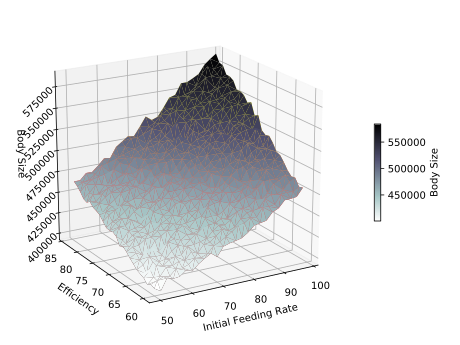
\includegraphics[trim = 0 0 150 50, clip, width=2.in, height=2.in]{C3/Figs/fr_eff/fr_eff_bs_MB}
}
\subfloat[MCU culture]{
  \centering
  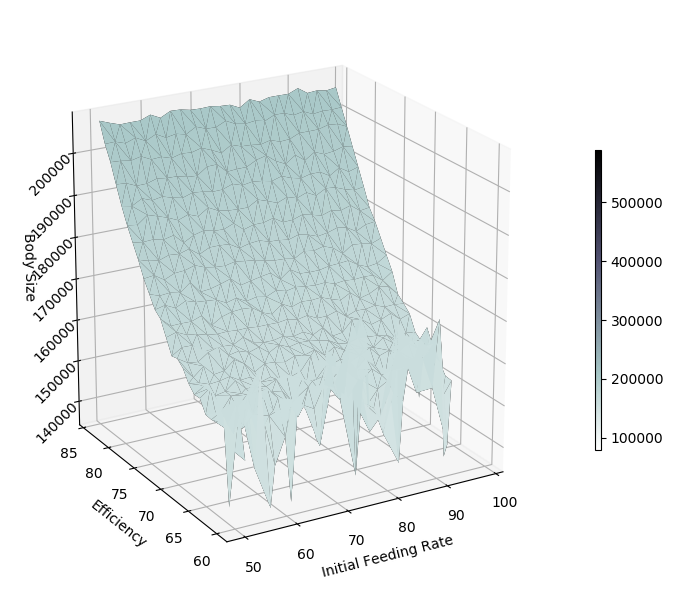
\includegraphics[trim = 0 0 150 50, clip, width=2.in, height=2.in]{C3/Figs/fr_eff/fr_eff_bs_MCU}
}
\subfloat[CCU culture]{
  \centering
  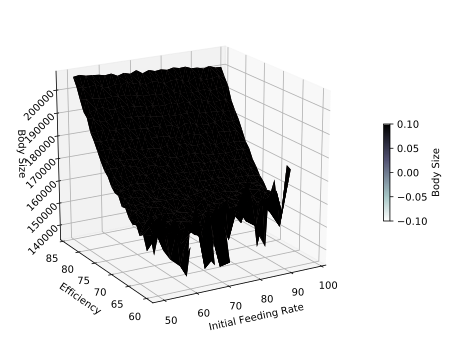
\includegraphics[trim = 0 0 0 50, clip, width=2.3in, height=2.in]{C3/Figs/fr_eff/fr_eff_bs_CCU}
}
\caption{Effect of initial feeding rate and efficiency on body size}
\label{fig:fr_eff_bs}
\end{figure}
\begin{figure}[p]
\subfloat[MB culture]{
  \centering
  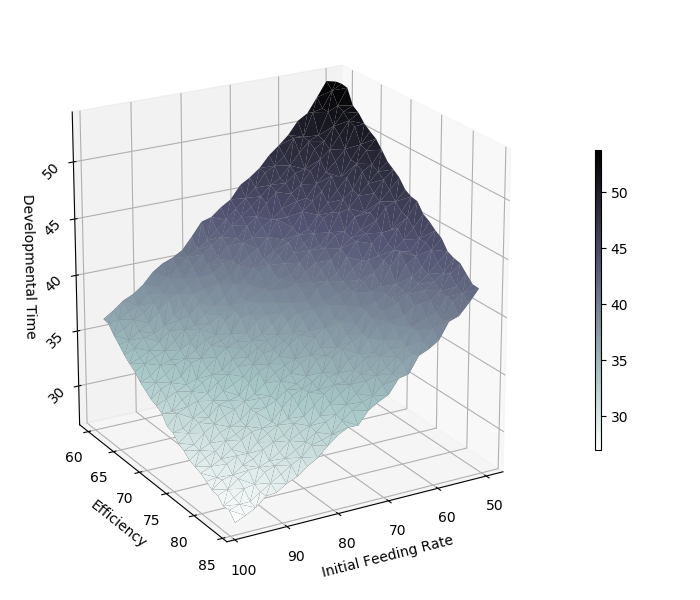
\includegraphics[trim = 0 0 150 50, clip, width=2.in, height=2.in]{C3/Figs/fr_eff/fr_eff_dt_MB}
}
\subfloat[MCU culture]{
  \centering
  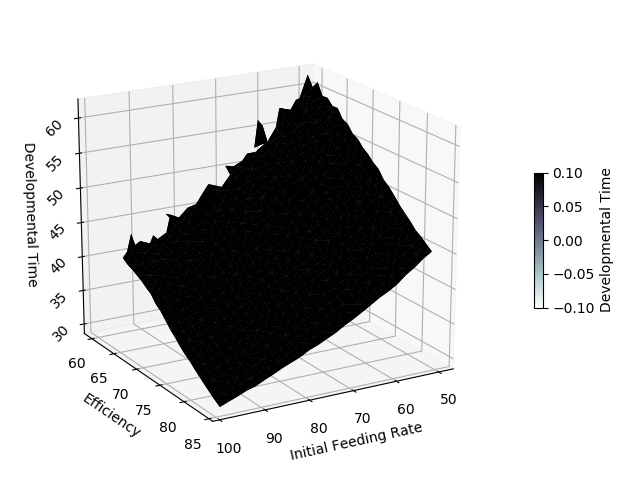
\includegraphics[trim = 0 0 150 50, clip, width=2.in, height=2.in]{C3/Figs/fr_eff/fr_eff_dt_MCU}
}
\subfloat[CCU culture]{
  \centering
  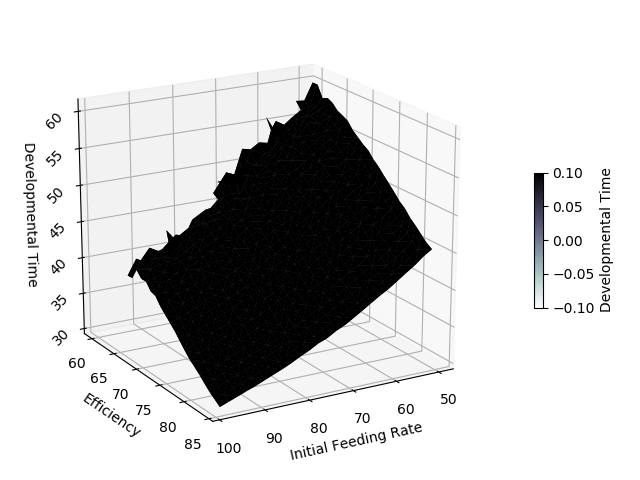
\includegraphics[trim = 50 0 0 50, clip, width=2.3in, height=2.in]{C3/Figs/fr_eff/fr_eff_dt_CCU}
}
\caption{Effect of initial feeding rate and efficiency on development time}
\label{fig:fr_eff_dt}
\end{figure}
\begin{figure}[p]
\subfloat[MB culture]{
  \centering
  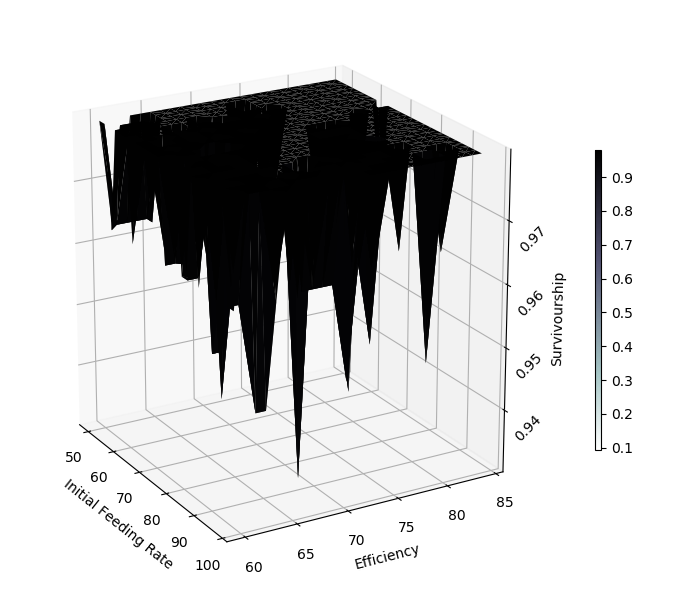
\includegraphics[trim = 50 0 100 50, clip, width=2.in, height=2.in]{C3/Figs/fr_eff/fr_eff_sur_MB}
}
\subfloat[MCU culture]{
  \centering
  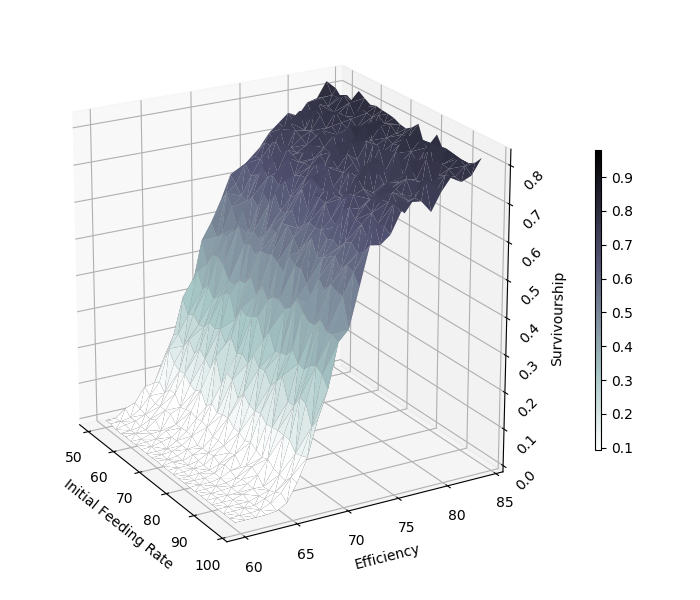
\includegraphics[trim = 50 0 100 50, clip, width=2.in, height=2.in]{C3/Figs/fr_eff/fr_eff_sur_MCU}
}
\subfloat[CCU culture]{
  \centering
  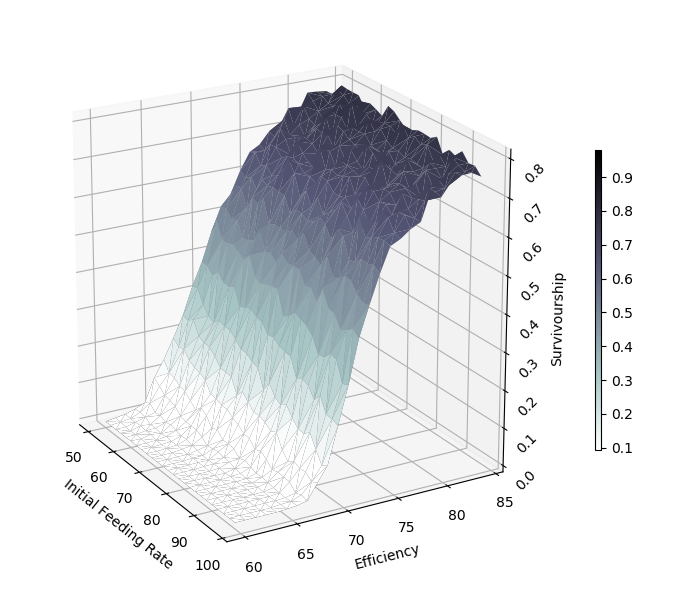
\includegraphics[trim = 0 0 0 50, clip, width=2.3in, height=2.in]{C3/Figs/fr_eff/fr_eff_sur_CCU}
}
\caption{Effect of initial feeding rate and efficiency on survivorship}
\label{fig:fr_eff_sur}
\end{figure}
\begin{figure}[p]
\subfloat[MB culture]{
  \centering
  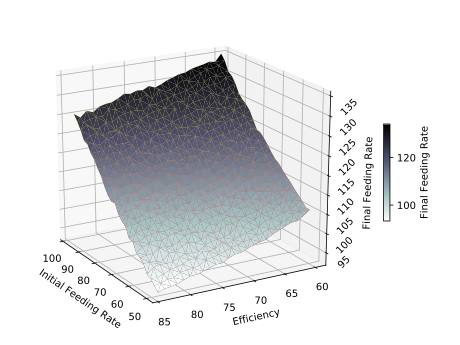
\includegraphics[trim = 0 0 150 50, clip, width=2.in, height=2.in]{C3/Figs/fr_eff/fr_eff_frt_MB}
}
\subfloat[MCU culture]{
  \centering
  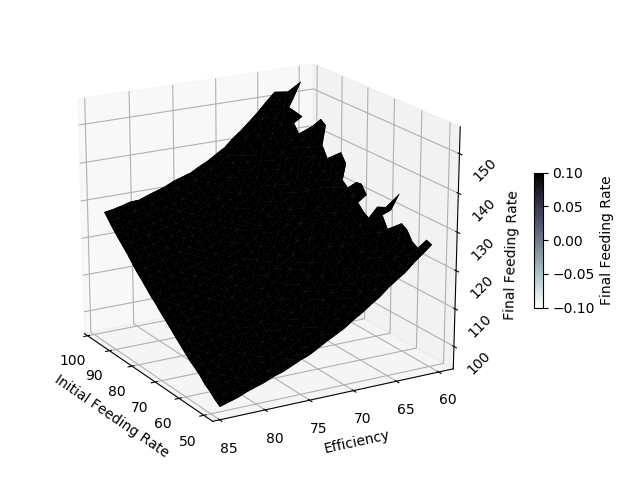
\includegraphics[trim = 0 0 150 50, clip, width=2.in, height=2.in]{C3/Figs/fr_eff/fr_eff_frt_MCU}
}
\subfloat[CCU culture]{
  \centering
  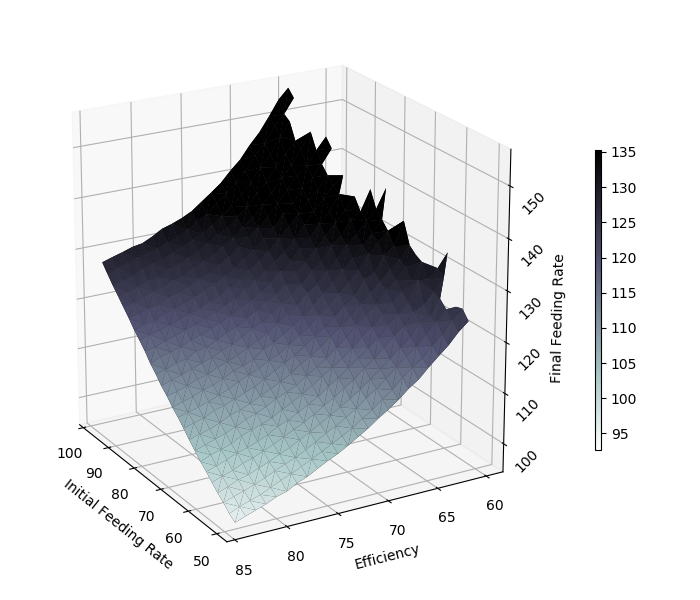
\includegraphics[trim = 0 0 0 50, clip, width=2.3in, height=2.in]{C3/Figs/fr_eff/fr_eff_frt_CCU}
}
\caption{Effect of initial feeding rate and efficiency on final feeding rate}
\label{fig:fr_eff_frt}
\end{figure}

\clearpage
\section{Initial Feeding Rate and Critical Size}
In simulations with varying mean trait values of initial feeding rate and critical size, all traits show a similar pattern with a varying density as seen with previous simulations. The larval body size shows similar correlations with initial feeding rate and critical size in MB and MCU culture, as seen in simulations varying initial feeding rate and efficiency (see fig~\ref{fig:fr_mc_bs}). In CCU culture, the body size is negatively correlated with initial feeding rate only for smaller values of critical size. However, it is not affected by initial feeding rate at larger critical size values. Fig~\ref{fig:fr_mc_dt} shows a negative correlation of development time with initial feeding rate, but a positive correlation with critical size in all culture vials. Survivorship is logistically dependent on critical size only in MCU and CCU culture. In MCU and CCU cultures, survivorship shows a slight negative correlation with initial feeding rate (see fig~\ref{fig:fr_mc_sur}). At all larval densities, final feeding rate is positively correlated with both initial feeding rate and critical size (see fig~\ref{fig:fr_mc_frt}).
\begin{figure}[hb]
\subfloat[MB culture]{
  \centering
  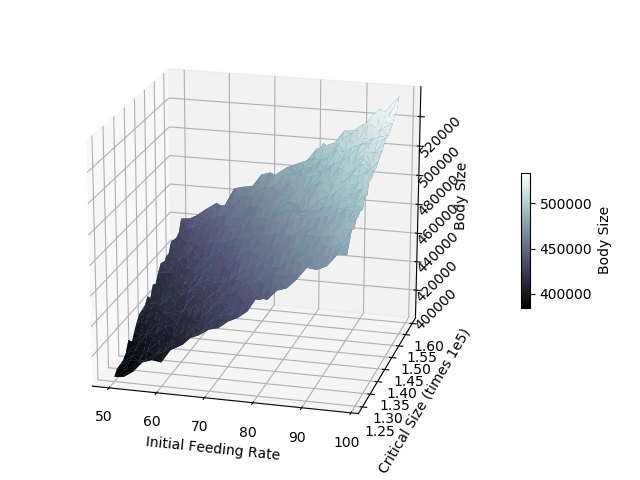
\includegraphics[trim = 0 0 150 50, clip, width=2.in, height=2.in]{C3/Figs/fr_mc/fr_mc_bs_MB}
}
\subfloat[MCU culture]{
  \centering
  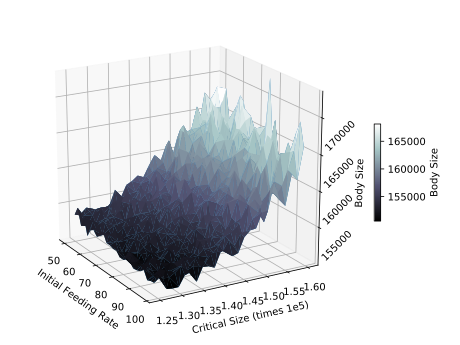
\includegraphics[trim = 0 0 150 50, clip, width=2.in, height=2.in]{C3/Figs/fr_mc/fr_mc_bs_MCU}
}
\subfloat[CCU culture]{
  \centering
  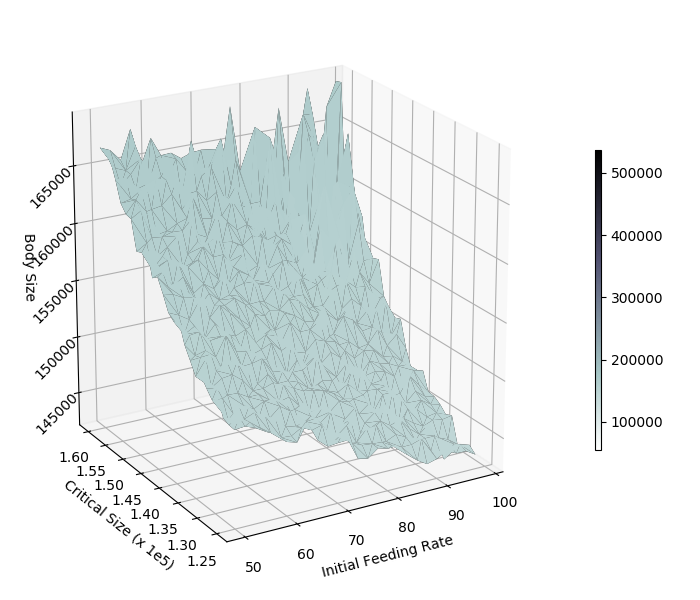
\includegraphics[trim = 0 0 0 50, clip, width=2.3in, height=2.in]{C3/Figs/fr_mc/fr_mc_bs_CCU}
}
\caption{Effect of initial feeding rate and critical size on body size}
\label{fig:fr_mc_bs}
\end{figure}
\begin{figure}[p]
\subfloat[MB culture]{
  \centering
  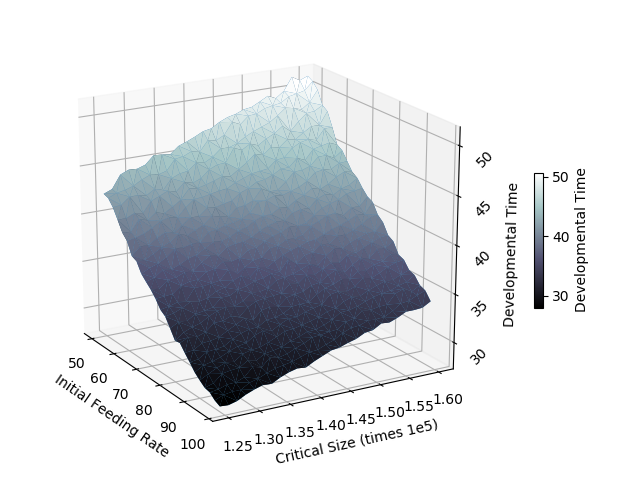
\includegraphics[trim = 50 0 100 50, clip, width=2.in, height=2.in]{C3/Figs/fr_mc/fr_mc_dt_MB}
}
\subfloat[MCU culture]{
  \centering
  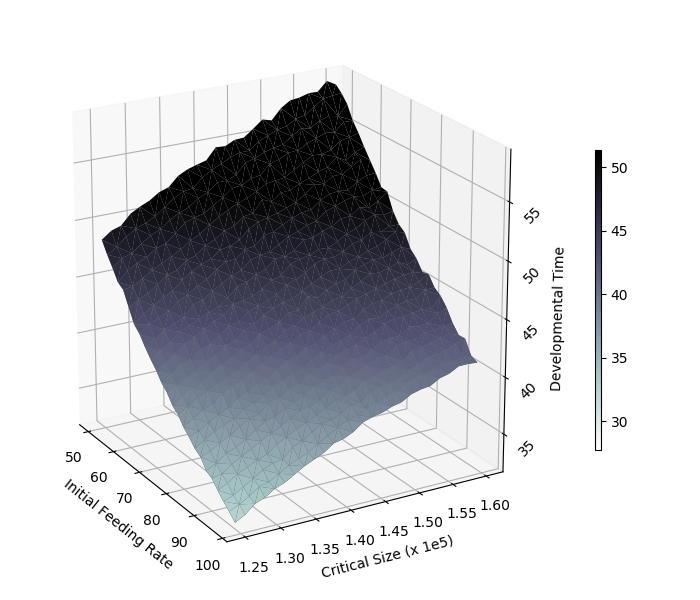
\includegraphics[trim = 50 0 100 50, clip, width=2.in, height=2.in]{C3/Figs/fr_mc/fr_mc_dt_MCU}
}
\subfloat[CCU culture]{
  \centering
  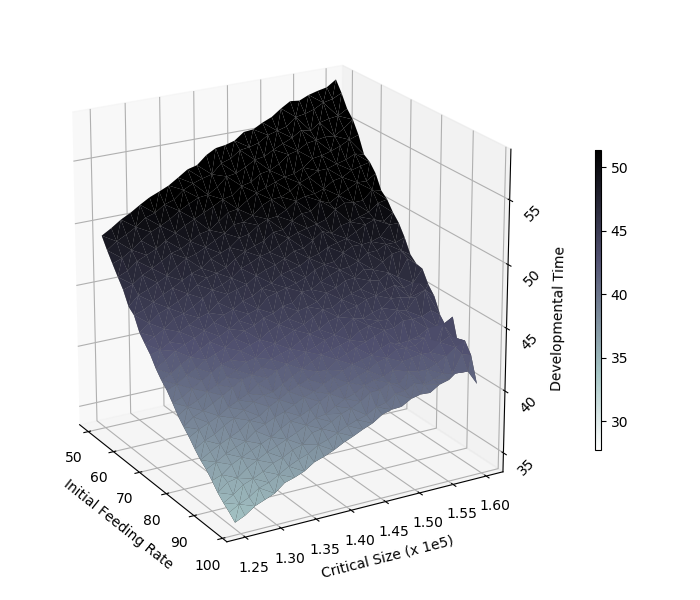
\includegraphics[trim = 0 0 0 50, clip, width=2.3in, height=2.in]{C3/Figs/fr_mc/fr_mc_dt_CCU}
}
\caption{Effect of initial feeding rate and critical size on development time}
\label{fig:fr_mc_dt}
\end{figure}
\begin{figure}[p]
\subfloat[MB culture]{
  \centering
  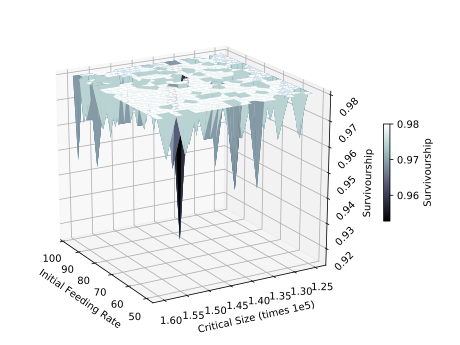
\includegraphics[trim = 0 0 150 50, clip, width=2.in, height=2.in]{C3/Figs/fr_mc/fr_mc_sur_MB}
}
\subfloat[MCU culture]{
  \centering
  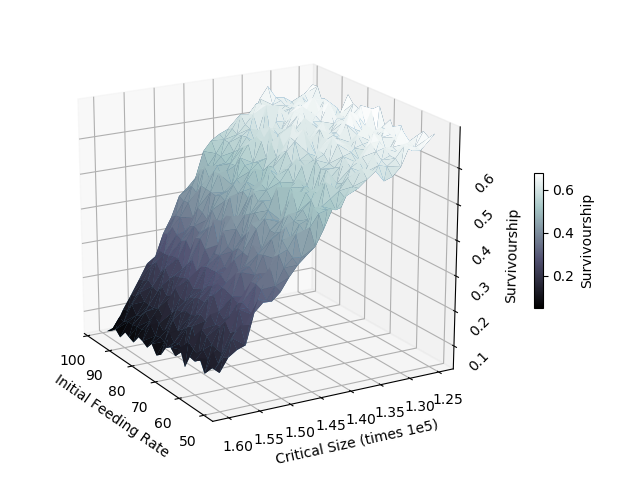
\includegraphics[trim = 0 0 150 50, clip, width=2.in, height=2.in]{C3/Figs/fr_mc/fr_mc_sur_MCU}
}
\subfloat[CCU culture]{
  \centering
  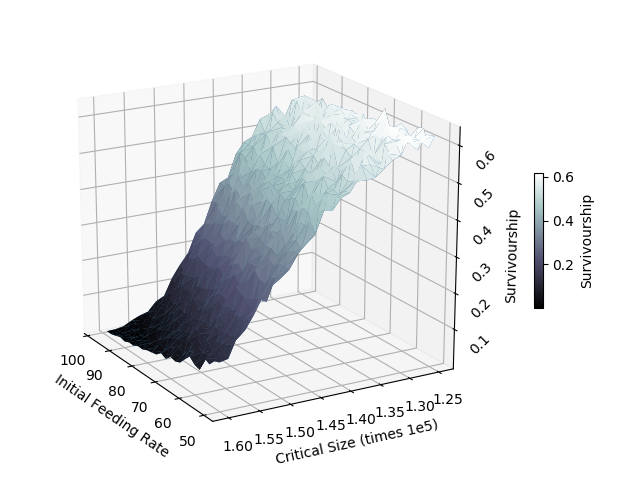
\includegraphics[trim = 0 0 0 50, clip, width=2.3in, height=2.in]{C3/Figs/fr_mc/fr_mc_sur_CCU}
}
\caption{Effect of initial feeding rate and critical size on survivorship}
\label{fig:fr_mc_sur}
\end{figure}

\begin{figure}[p]
\subfloat[MB culture]{
  \centering
  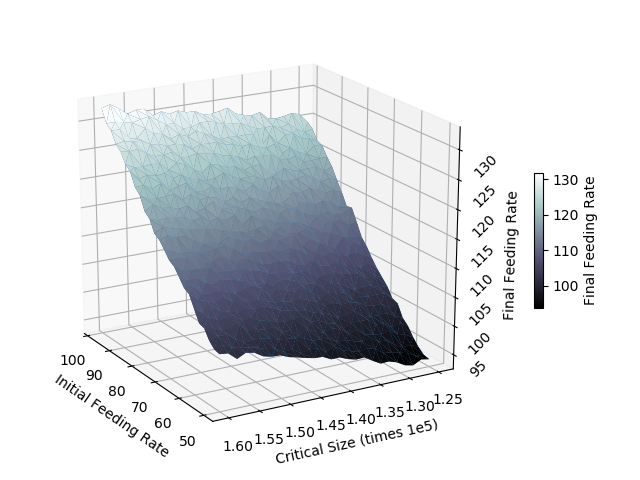
\includegraphics[trim = 0 0 150 50, clip, width=2.in, height=2.in]{C3/Figs/fr_mc/fr_mc_frt_MB}
}
\subfloat[MCU culture]{
  \centering
  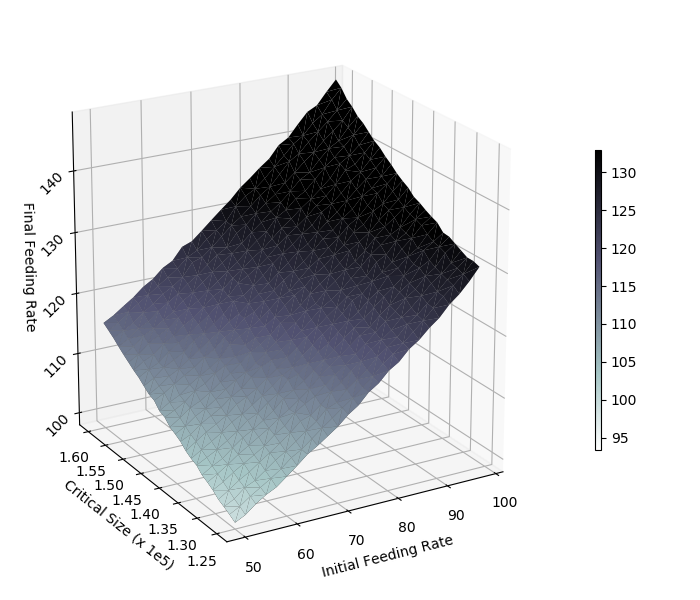
\includegraphics[trim = 0 0 150 50, clip, width=2.in, height=2.in]{C3/Figs/fr_mc/fr_mc_frt_MCU}
}
\subfloat[CCU culture]{
  \centering
  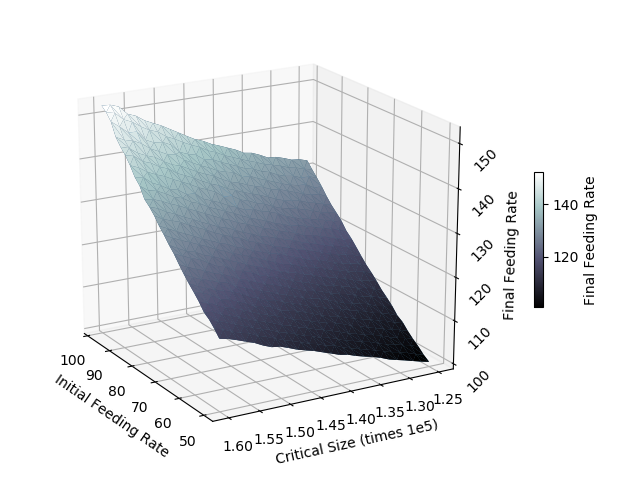
\includegraphics[trim = 0 0 0 50, clip, width=2.3in, height=2.in]{C3/Figs/fr_mc/fr_mc_frt_CCU}
}
\caption{Effect of initial feeding rate and critical size on final feeding rate}
\label{fig:fr_mc_frt}
\end{figure}

\clearpage
\section{Critical Size and Efficiency}
In simulations varying mean trait values of critical size and efficiency, all larval traits measured show again a similar pattern with density. The larval body size shows similar correlations with critical size and efficiency in MB culture, as seen in previous simulations, varying initial feeding rate and efficiency (see fig~\ref{fig:mc_eff_bs}). In MCU and CCU cultures, the body size is positively correlated with critical size only for smaller values of efficiency. However, it is not affected by a critical size at larger efficiency values. Fig~\ref{fig:mc_eff_dt} shows a negative correlation of development time with efficiency, but positive correlation with critical size at all densities. Survivorship is again logistically dependent on efficiency only in MCU and CCU culture. In MCU and CCU cultures, survivorship also shows a negative correlation with critical size at lower values of efficiency (see fig~\ref{fig:mc_eff_sur}). At all larval densities, final feeding rate is positively correlated with critical size and negatively with efficiency (see fig~\ref{fig:mc_eff_frt}).
\begin{figure}[hb]
\subfloat[MB culture]{
  \centering
  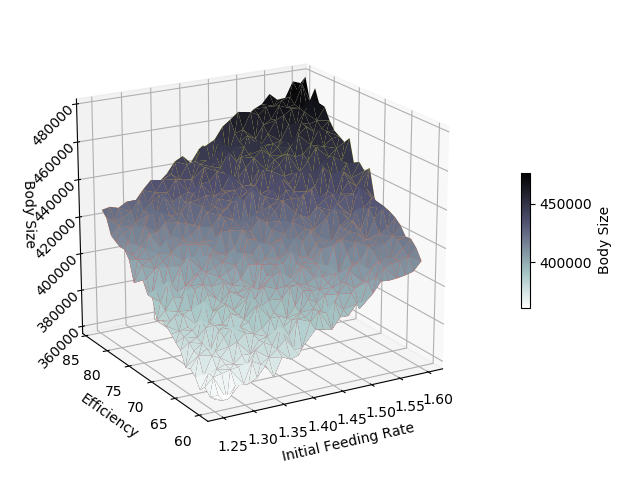
\includegraphics[trim = 0 0 150 50, clip, width=2.in, height=2.in]{C3/Figs/mc_eff/mc_eff_bs_MB}
}
\subfloat[MCU culture]{
  \centering
  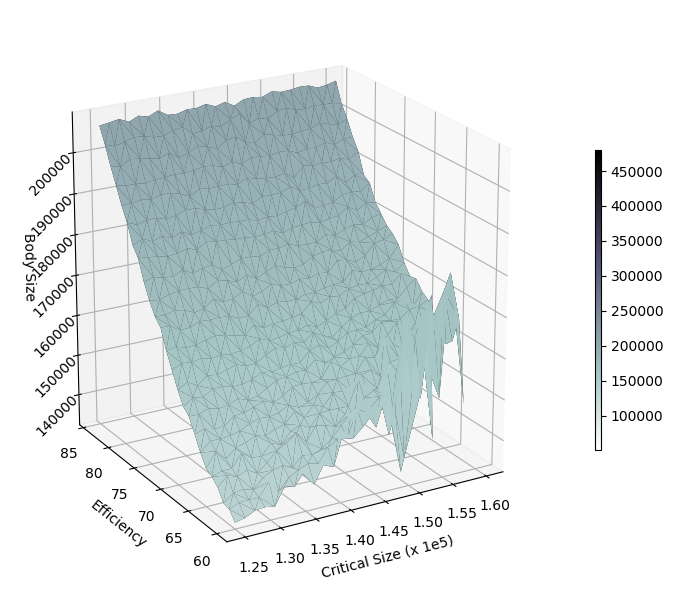
\includegraphics[trim = 0 0 150 50, clip, width=2.in, height=2.in]{C3/Figs/mc_eff/mc_eff_bs_MCU}
}
\subfloat[CCU culture]{
  \centering
  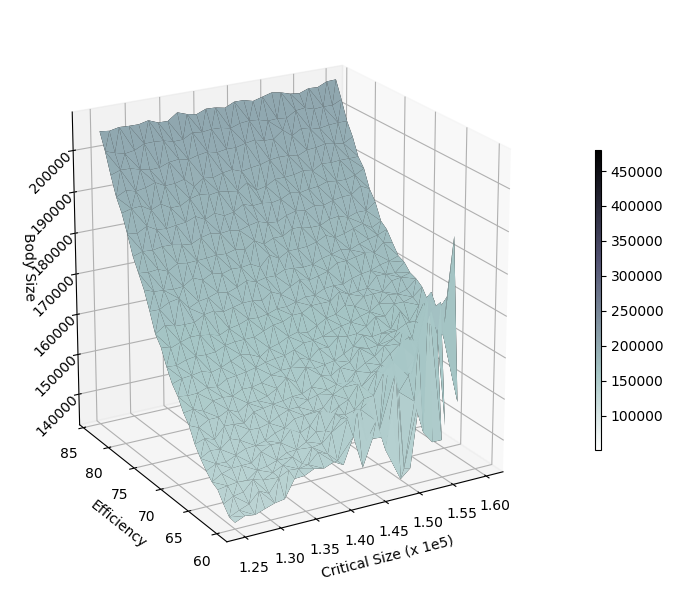
\includegraphics[trim = 0 0 0 50, clip, width=2.3in, height=2.in]{C3/Figs/mc_eff/mc_eff_bs_CCU}
}
\caption{Effect of critical size and efficiency on body size}
\label{fig:mc_eff_bs}
\end{figure}

\begin{figure}[p]
\subfloat[MB culture]{
  \centering
  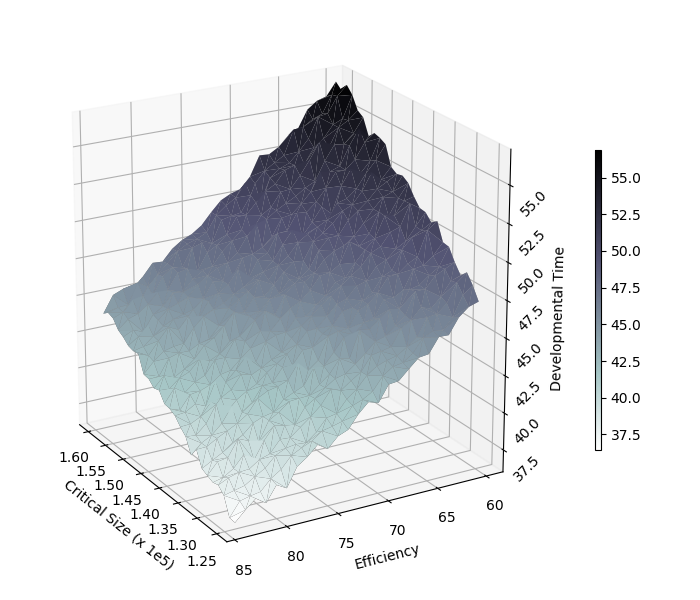
\includegraphics[trim = 50 0 100 50, clip, width=2.in, height=2.in]{C3/Figs/mc_eff/mc_eff_dt_MB}
}
\subfloat[MCU culture]{
  \centering
  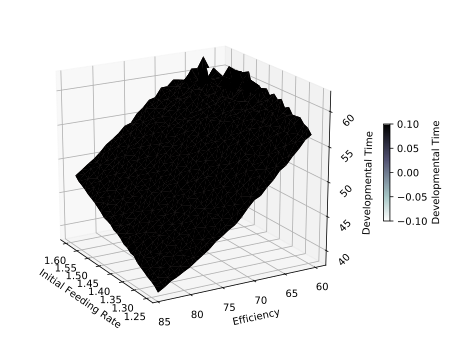
\includegraphics[trim = 50 0 100 50, clip, width=2.in, height=2.in]{C3/Figs/mc_eff/mc_eff_dt_MCU}
}
\subfloat[CCU culture]{
  \centering
  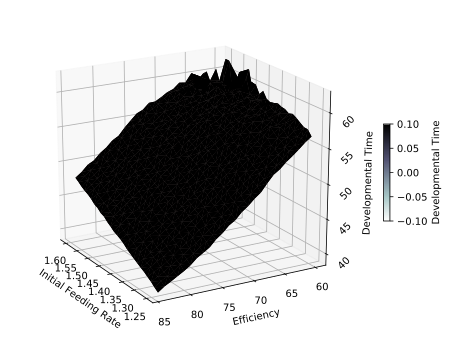
\includegraphics[trim = 0 0 0 50, clip, width=2.3in, height=2.in]{C3/Figs/mc_eff/mc_eff_dt_CCU}
}
\caption{Effect of critical size and efficiency on development time}
\label{fig:mc_eff_dt}
\end{figure}

\begin{figure}[p]
\subfloat[MB culture]{
  \centering
  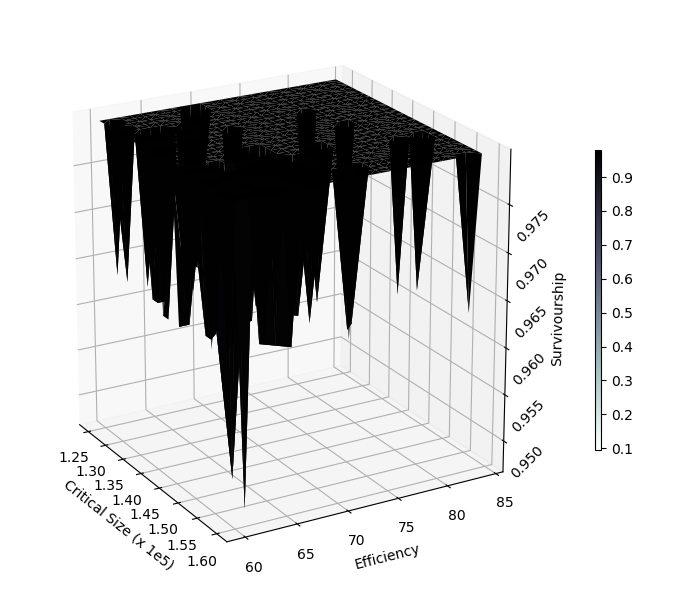
\includegraphics[trim = 0 0 150 50, clip, width=2.in, height=2.in]{C3/Figs/mc_eff/mc_eff_sur_MB}
}
\subfloat[MCU culture]{
  \centering
  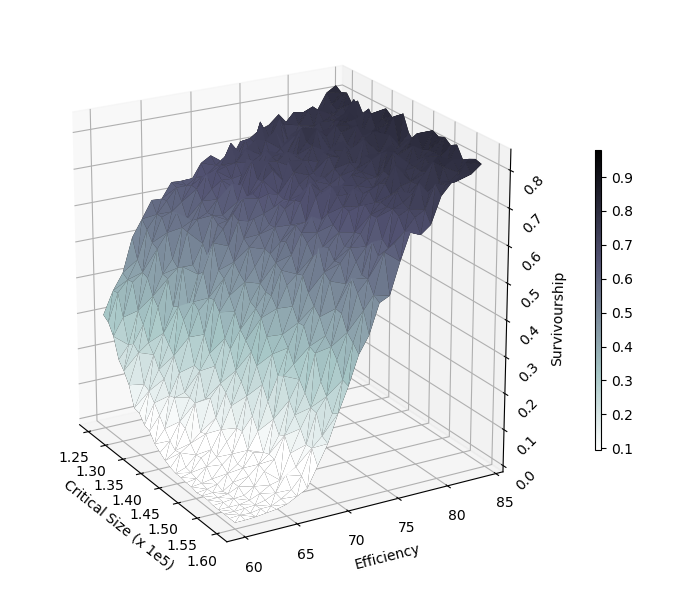
\includegraphics[trim = 0 0 150 50, clip, width=2.in, height=2.in]{C3/Figs/mc_eff/mc_eff_sur_MCU}
}
\subfloat[CCU culture]{
  \centering
  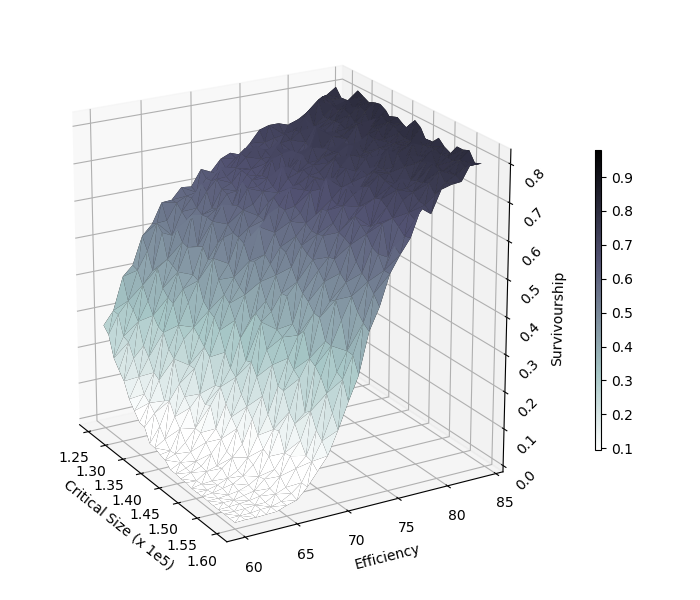
\includegraphics[trim = 0 0 0 50, clip, width=2.3in, height=2.in]{C3/Figs/mc_eff/mc_eff_sur_CCU}
}
\caption{Effect of critical size and efficiency on survivorship}
\label{fig:mc_eff_sur}
\end{figure}

\begin{figure}[p]
\subfloat[MB culture]{
  \centering
  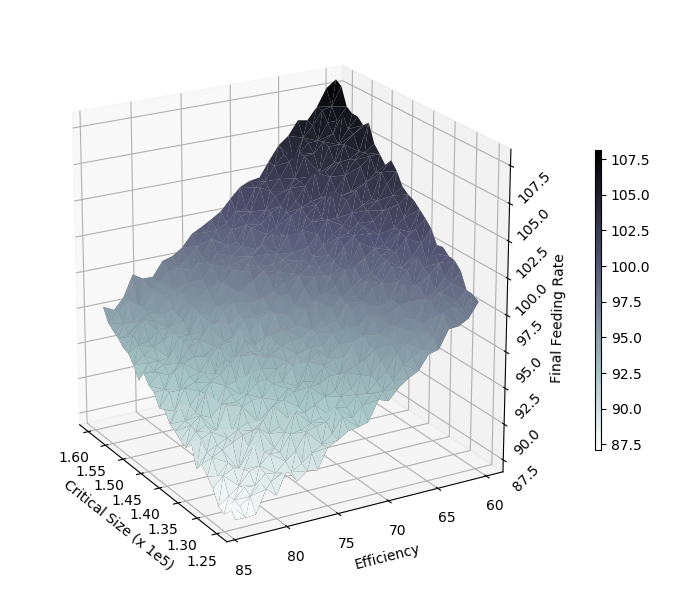
\includegraphics[trim = 0 0 150 50, clip, width=2.in, height=2.in]{C3/Figs/mc_eff/mc_eff_frt_MB}
}
\subfloat[MCU culture]{
  \centering
  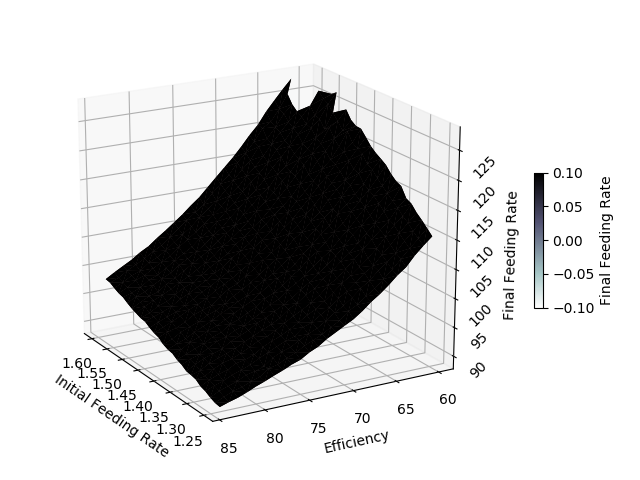
\includegraphics[trim = 0 0 150 50, clip, width=2.in, height=2.in]{C3/Figs/mc_eff/mc_eff_frt_MCU}
}
\subfloat[CCU culture]{
  \centering
  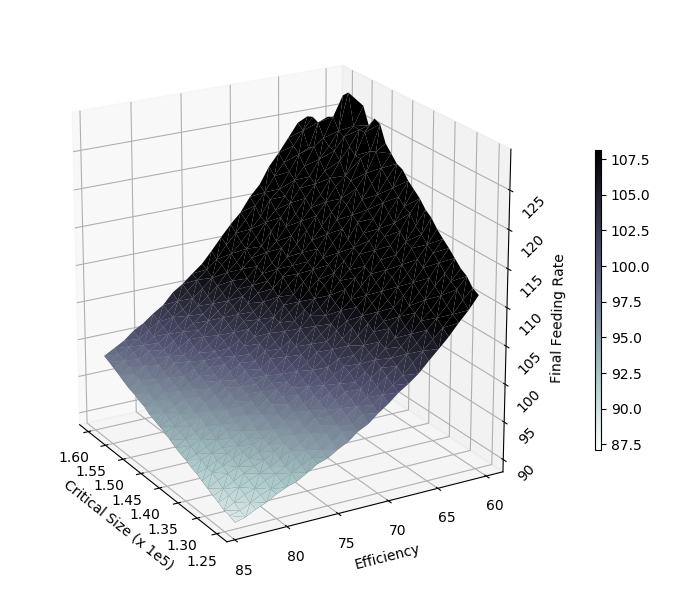
\includegraphics[trim = 0 0 0 50, clip, width=2.3in, height=2.in]{C3/Figs/mc_eff/mc_eff_frt_CCU}
}
\caption{Effect of critical size and efficiency on final feeding rate}
\label{fig:mc_eff_frt}
\end{figure}
\pagebreak
